\chapter{Elastyczne indeksowanie}

Termin ``elastyczne indeksowanie'' (\emph{flexible indexing}) określa nowe podejście do architektury Lucene, wprowadzone w wersji 4.0. Polega ono na oddzieleniu formatu indeksu (fizycznego sposobu zapisu poszczególnych jego elementów na dysku) od logicznych operacji na nim wykonywanych.

\section{Cel wprowadzenia zmian}

W październiku 2012 roku, po ok. dwóch latach prac, została opublikowana wersja 4.0 Lucene, znacząco różniąca się od poprzednich -- głównie dzięki wprowadzeniu tzw. \emph{architektury kodekowej}. Części biblioteki odpowiedzialne za indeksowanie zostały logicznie wydzielone i umieszczone w dodatkowej warstwie architektury (kodeku). 

Głównym powodem wprowadzenia zmian był przestarzały i nieelastyczny format kodowania indeksu. Wersje 3.x Lucene oraz wcześniejsze do zapisu list postingowych posługiwały się formatem \texttt{vInt} -- liczb całkowitych o zmiennej długości bitowej. Format ten był ściśle związany z wszystkimi częściami kodu. W związku z tym jakakolwiek jego modyfikacja wymagała sporego nakładu pracy programisty. Utrudniało to rozwój Lucene oraz eksperymentowanie z nowymi sposobami kompresji czy strukturami danych. Format \texttt{vInt} istniał w Lucene praktycznie od jej początków (ok. 10 lat, od wersji 1.0). Od tego czasu powstały efektywniejsze algorytmy kompresji.

Stara architektura uniemożliwiała także zapis dodatkowych statystyk do indeksu -- co utrudniało (lub uniemożliwiało) implementacje nowych algorytmów obliczania miar dopasowania dokumentu do zapytania.

Lucene, pomimo, że była najpopularniejszym narzędziem do wyszukiwania tekstowego stosowanym w komercyjnych projektach, rzadko była wykorzystywana w środowiskach naukowych -- właśnie ze względu na brak możliwości łatwych zmian formatów indeksu i eksperymentowania na nim. Nowa architektura miała to zmienić: umożliwić bardziej elastyczny rozwój przy jednoczesnym zachowaniu wydajności.

\section{Architektura oparta o kodeki}

Zmiany architektury polegały na wprowadzeniu dodatkowej warstwy pośredniczącej pomiędzy formatem dyskowym indeksu a biblioteką. Ilustruje to rysunek ~\ref{newarchitecture} (źródło: \cite{flexindex}).

\begin{figure}[here]
 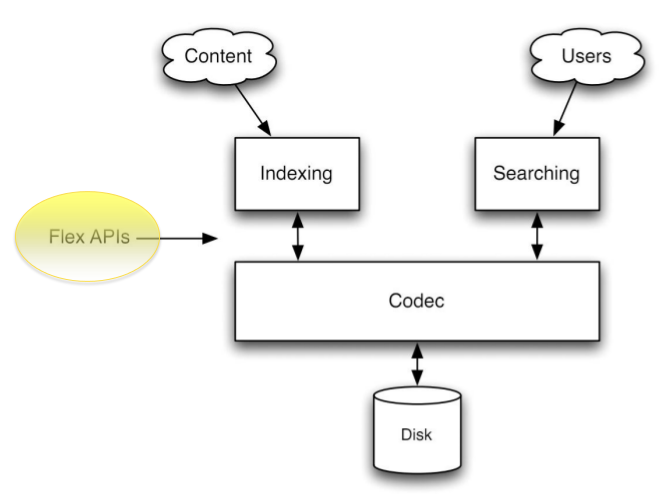
\includegraphics[scale=0.5]{architecture.png}
 \caption{Schemat architektury opartej o kodeki.}
 \label{newarchitecture}
\end{figure}

Operacje na indeksie (dodawanie, usuwanie lub modyfikowanie dokumentów, wyszukiwanie) są implementowane w wyższych warstwach biblioteki. Kodek dostarcza formatu narzędzi do zapisu i odczytu danych o zaindeksowanych dokumentach. Poprzez jego podmianę można zastosować np. niestandardowe algorytmy kompresji, struktury danych do przechowywania słowników termów itp.

\section{Struktura kodeka}

Każdy kodek składa się z ośmiu części. Istnieje możliwość łączenia istniejących rozwiązań z własnymi implementacjami. Oznacza to, że można skorzystać z domyślnych implementacji większości tych elementów i podmienić np. tylko część odpowiedzialną za kodowanie list postingowych.

Elementy, na które składa się kodek to:
\begin{enumerate}
 \item format list postingowych,
 \item format DocValues,
 \item format pól przechowywanych (\emph{stored fields}),
 \item format dla \emph{term vectors},
 \item format informacji o polach i związanych z tym statystyk (\emph{field infos format}),
 \item format zapisu ogólnych informacji dotyczących segmentów (\emph{segment info format}),
 \item format zapisu norm -- związanych z poszczególnymi polami liczb wskazujących, czy dane pole powinno być traktowane jako mniej lub bardziej istotne niż pozostałe (wskaźniki \emph{boost} zapisywanie podczas indeksowania),
 \item format do zapisu informacji o tym, które dokumenty powinny zostać usunięte podczas najbliższej optymalizacji indeksu (\emph{live docs format}).
\end{enumerate}

\section{Czterowymiarowa struktura indeksu}

Zmiany, poza rozdzieleniem formatu zapisu indeksu do plików od architektury, dotyczyły także interfejsu programisty. Dostęp do poszczególnych elementów indeksu, czyli pól, termów, numerów dokumentów, pozycji wystąpień termu w dokumencie, itp. odbywa się przy pomocy tzw. czterowymiarowego API, które obrazowo przedstawione jest na rys. ~\ref{4dimAPI} (żródło: \cite{flexindex}).

\begin{figure}[here]
 \label{4dimAPI}
 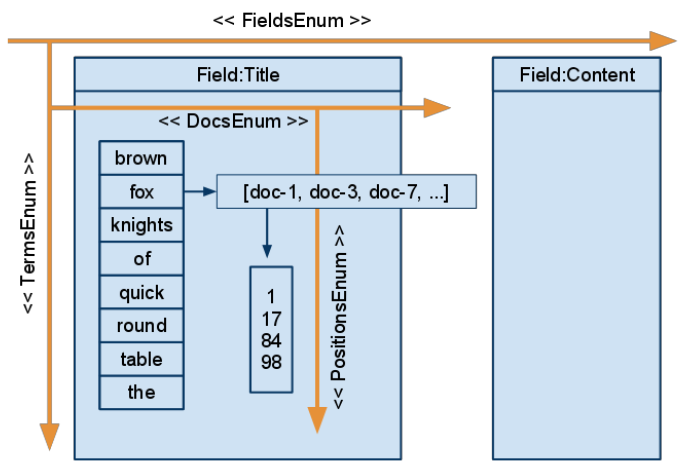
\includegraphics[scale=0.5]{api.png}
 \caption{Schemat interfejsu programisty pozwalającego na dostęp do poszczególnych elementów indeksu.}
\end{figure}

Najbardziej nadrzędnym elementem dostępu do indeksu jest pole (\texttt{Field}). W uproszczeniu, dla każdego indeksu (bądź jego abstrakcji) możemy pobrać listę jego pól (\texttt{FieldsEnum}). Pole, poza tytułem, posiada listę termów, do której mamy dostęp poprzez iterator \texttt{TermsEnum}. Dla każdego termu możemy pobrać listę dokumentów, w których on wystąpił (\texttt{DocsEnum}), a dla każego z dokumentów -- listę pozycji wystąpień (\texttt{PositionsEnum}).

Powyższy schemat jest dość uproszczony i nie oddaje faktycznej struktury klas. Rysunek poniżej ilustruje, w jaki sposób koncepcja czterowymiarowego API została przełożona na abstrakcyjne klasy Lucene Core. Programista chcący zaimplementować własny kodek musi stworzyć swoją hierarchię klas zgodnie z tą strukturą.

\begin{figure}[here]
 \label{indexApi}
 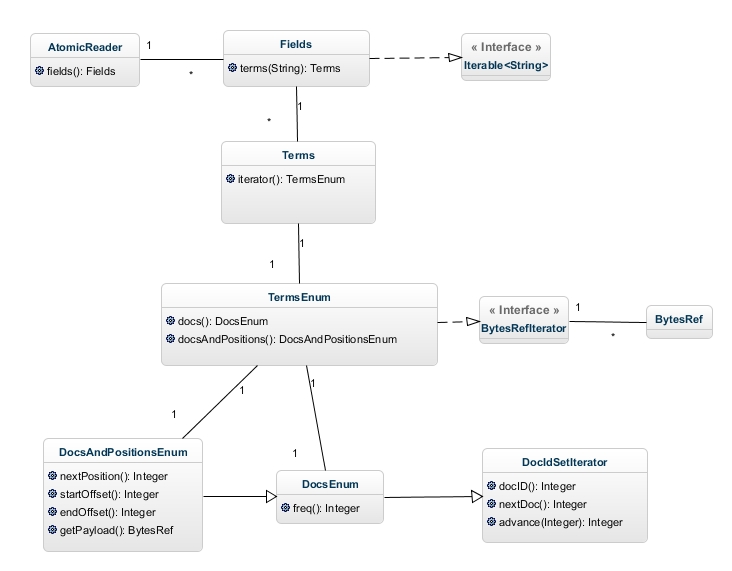
\includegraphics[scale=0.6]{LuceneAccessAPI.jpg}
 \caption{Struktura klas służących do pobierania poszczególnych elementów indeksu. Źródło: opracowanie własne.}
\end{figure}

Pola są najwyższą warstwą w hierarchii dostępu do danych indeksu. Dodatkowo, istnieje możliwość skonfigurowania, który kodek powinien być używany do wskazanego pola. Możemy więc myśleć o indeksie zawierającym wiele pól jako o kilku równoległych indeksach. To także ma wpływ na sposób traktowania termów: ten sam term, ale znajdujący się w dwóch różnych polach jest traktowany jako dwa osobne termy. 

\texttt{AtomicReader} jest abstrakcyjnym rozszerzeniem \texttt{IndexReadera}. Dostarcza interfejsu dostępu do pól przechowywanych w indeksie: potrafi zwrócić obiekt \texttt{Fields}, implementujący interfejs iteratora napisów. Oznacza to, że \texttt{Fields.iterator()} przechodzi po wszystkich nazwach pól znajdujących się w indeksie. Więcej informacji na temat wykorzystania, struktury i powiązań pomiędzy poszczególnymi implementacjami \texttt{IndexReader} znajduje się w sekcji \ref{sec:indexReader}.

Z obiektu \texttt{Fields} można pobrać obiekt \texttt{Terms}, który poza iteratorem termów (\texttt{TermsEnum}) zawiera także statystyki dotyczące wszystkich termów pola (liczba dokumentów, w których ten term występuje, łączna liczba wystąpień termu w polu).

Od wersji 4.0 Lucene term jest reprezentowany jako ciąg bajtów (a nie, jak wcześniej, jako napis w kodowaniu UTF-16). Pozwala to na uniknięcie problemów związanych z kodowaniem znaków, szczególnie w językach wschodnioazjatyckich -- odpowiedzialność za kodowanie i odkodowywanie znaków z ciągu bajtów jest przerzucona na kodek. Klasą wykorzystaną do reprezentacji takiego ciągu jest \texttt{BytesRef} (który tak naprawdę przechowuje informacje o początku danego podciągu oraz jego długości w większej tablicy typu \texttt{byte[]}).

Zauważmy, że \texttt{TermsEnum} implementuje interfejs \texttt{BytesRefIterator}. Oznacza to tyle, że jest on w stanie wylistować wszystkie przechowywane termy. Tę samą funkcjonalność można byłoby uzyskać wykorzystując standardowy iterator dla Javy (\texttt{TermsEnum} mogłoby implementować \texttt{Iterable<BytesRef>}). Wygląda na to, że wprowadzanie dodatkowej klasy, \texttt{BytesRefIterator}, jest niepotrzebne i powoduje tylko spadek czytelności kodu.

W zależności od tego, czy podczas indeksowania dla każdego wystąpienia termu zostały zapisane dodatkowe informacje (pozycje wystąpień, \emph{payloads}), do wylistowania dokumentów, w których wystąpił dany term można użyć jednej z dwóch abstrakcji: \texttt{DocsEnum} lub rozszerzającego \texttt{DocsAndPositionsEnum}. 

Zauważmy, że do wylistowania wszystkich dokumentów z \texttt{DocsEnum} wykorzystany jest kolejny interfejs iteratora: \texttt{DocIdSetIterator}. W tym wypadku wprowadzenie dodatkowej klasy dla tej samej funkcjonalności wydaje się jednak uzasadnione: \texttt{DocIdSetIterator}, poza standardowymi funkcjami iteratora, pozwala na przejście do wskazanego elementu listy (abstrakcyjne metody \texttt{advance(int target)} oraz \texttt{slowAdvance(int target)}: dokumentacja sugeruje, aby implementacja pierwszej z nich wykorzystywała skip listy).

\section{Dostęp do plików indeksu: \texttt{IndexReader} i jego implementacje}
\label{sec:indexReader}

\section{Implementacja własnego kodeka}

Format list postingowych jest miejscem, które najprawdopodobniej chciałby zmienić programista chcący zaimplementować np. nowy algorytm kompresji. Dlatego zajmiemy się teraz opisem architektury tej części kodeka. 

Aby zaimplementować własny kodek, należy przeciążyć abstrakcyjną klasę \texttt{Codec}, gromadzącą poszczególne elementy kodeka (formaty). Za format list postingowych odpowiada klasa \texttt{PostingsFormat}. Jej głównym zadaniem jest dostarczenie i zarządzanie cyklem życia dwóch obiektów: \texttt{FieldsProducer} i \texttt{FieldsConsumer}, które są odpowiedzialne za, odpowiednio odczyt i zapis danych z plików indeksu. Architekturę formatu list postingowych przedstawia rys. \ref{postingFormat}.

\begin{figure}[here]
 \label{postingFormat}
 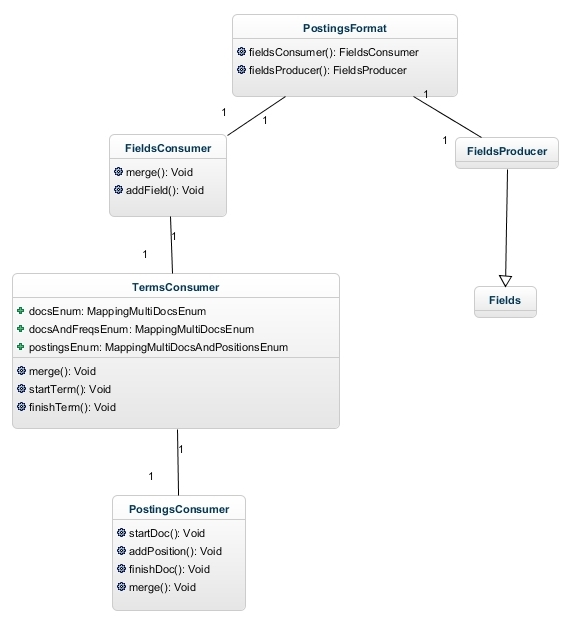
\includegraphics[scale=0.6]{PostingsFormat.jpg}
 \caption{Schemat klas służących do zapisu formatu list postingowych.}
\end{figure}

Klasa \texttt{FieldsProducer} jest odpowiedzialna za odczyt danych z segmentu -- stąd powiązanie z przedstawioną już wcześniej klasą \texttt{Fields}. \texttt{FieldsConsumer} jest z kolei odpowiedzialny za zapis nowego segmentu (powstałego w wyniku zrzutu danych na dysk lub w wyniku łączenia segmentów). Określenia \emph{producer} i \emph{consumer} mogą wydawać się tutaj mało intuicyjne. Zrozumienie ich ról może ułatwić następujące zdanie: ,,\texttt{FieldsConsumer} \emph{pobiera} (konsumuje) właśnie definiowane pole i zapisuje je w indeksie, podczas gdy \texttt{FieldsProducer} odczytuje pole z indeksu (\emph{produkuje} je z plików indeksu)''.

Dodawanie nowych pól do instancji \texttt{FieldsConsumera} odbywa się za pomocą metody \texttt{addField()} przyjmującej jako parametr obiekt typu \texttt{FieldInfo}, przechowujący informacje o konfiguracji pola (takie jak jego wewnętrzny numer, nazwę, opcje indeksowania, atrybuty, itp.). Metoda ta zwraca obiekt \texttt{TermsConsumer}, pozwalający na dodawanie termów do pola. \texttt{TermsConsumer} posiada trzy atrybuty typu \texttt{DocsEnum} (a konkretniej: typów rozszerzających \texttt{DocsEnum}). Są one wykorzystywane podczas łączenia segmentów -- w zależności od opcji indeksowania, wybierane jest jedno a nich i ono pełni rolę iteratora dokumentów.

Wywołanie \texttt{TermsConsumer.startTerm()} zwraca obiekt \texttt{PostingsConsumer}, który, operując już na numerach dokumentów i pozycjach występowania danego termu, zapisuje listy postingowe.

Oczywiście, wszystkie klasy diagramu \ref{fig:postingFormat} są abstrakcyjne -- wszystkie wymienione operacje (takie jak dodawanie pola, termu lub dokumentu) muszą być oprogramowane w klasach kodeka. Klasy \texttt{FieldsConsumer}, \texttt{TermsConsumer}, \texttt{PostingsConsumer} posiadają jedynie implementacje metod \texttt{merge()}. Według projektantów Lucene łączenie poszczególnych elementów indeksu powinno być niezależne od faktycznego formatu zapisu. Nic jednak nie stoi na przeszkodzie, aby kodek nadpisywał także tę funkcjonalność.

Jedyną zaimplementowaną funkcjo

\section{Format list postingowych}

Format list postingowych zależy od kodeka. Przedstawiony tutaj zostanie obecnie stosowany format, dla domyślnego kodeka używanego w Lucene od wersji 4.1.

Elementami list postingowych są różnice pomiędzy numerami dokumentów. Na liście postingowej może być dodatkowo przechowywana informacja o liczbe wystąpień danego termu w dokumencie.

Listy postingowe kodowane są blokami dwóch rodzajów. Wszystkie bloki (być może poza ostatnim) są blokami tzw. upakowanymi (\emph{Packed Blocks}). Liczba postingów w takim bloku jest stała i wynosi 128. Jeśli liczba postingów w liście nie jest podzielna przez 128, pozostałe postingi (te, które nie zmieściły się w ostatnim bloku upakowanym) są zapisywane w postaci osobnego bloku i są kodowane przy pomocy liczb całkowitych o zmiennej długości (tzw. \emph{vInt format}).

Lista postingowa jest skip listą: istnieje możliwość ,,przeskakiwania'' o całe bloki. Wskaźniki skip list zapisywane są na począteku każdego bloku (z wyjątkiem pierwszego).

\subsection{Kodowanie bloków upakowanych}

Każdy blok upakowany (\emph{PackedBlock}) składa się z dwóch części: 
\begin{enumerate}
 \item upakowanych numerów dokumentów (\emph{PackedDocDeltaBlock}),
 \item (opcjonalnie) części kodującej częstości wystąpienia danego termu w dokumencie (\emph{PackedFreqBlock}).
\end{enumerate}

Algorytm kodowania numerów dokumentów w bloku upakowanym jest bardzo prosty: najpierw obliczane są różnice pomiędzy kolejnymi numerami dokumentów (tzw. \emph{d-gaps}), a następnie kolejne grupy po 128 postingów są osobno kodowane jako blok upakowany. Dla każdej grupy \emph{d-gaps}, która ma zostać zakodowana jako blok, wybierana jest minimalna liczba bitów, przy pomocy której wszystkie z nich będą mogły zostać zakodowane. Informacja o tej liczbie zapisywana jest w pierwszym bajcie bloku. Następnie zapisywany jest ciąg zakodowanych \emph{d-gaps}.

Dodatkowo, jeśli wszystkie \emph{d-gaps} są takie same (np. jeśli dany term występuje we wszystkich dokumentach i w związku z tym wszystkie \emph{d-gaps} mają wartość 1), w pierwszym bajcie bloku zapisywana jest wartość 0, a następnie -- powtarzająca się liczba jako pojedynczy \texttt{vInt}.

Wedle tego podobnego schematu kodowana jest część zawierająca częstości wystąpień termu w dokumencie -- z pominięciem obliczania \emph{d-gaps}, które tutaj nie są potrzebne.

\subsection{Kodowanie \texttt{vInt}}

W tym formacie kodowania informacje o numerze dokumentu oraz o częstości występowania termu są zakodowane naprzemiennie (tzn. jeśli częstość występowania termu w danym dokumencie jest większa niż 1, kodowana jest jako kolejna liczba na liście). 

Elementy tego bloku nazywane się \emph{DocDelta} i kodowane są jako liczby \texttt{vInt}. Kodowaniem tym rządzą następujące reguły:
\begin{itemize}
 \item jeśli częstości występowania termu są zaindeksowane, wartość \emph{DocDelta} zawiera informacje zarówno o \emph{d-gap} jak i o częstości,
 \item $\emph{d-gap} = \emph{DocDelta} / 2$ (dzielenie bez reszty)
 \item jeśli $\emph{DocDelta}~\%~2 = 1$, to częstość termu wynosi 1,
 \item jeśli $\emph{DocDelta}~\%~2 = 0$, to częstość występowania termu zakodowana jest jako kolejna liczba (\texttt{vInt}) na liście.
\end{itemize}

Kodowanie liczb \texttt{vInt} (liczb całkowitych o zmiennej długości) odbywa się tak, jak opisano w \cite{irbook} w rozdziale 5.3.1 ,,Variable byte encodes''. Pierwszy bit każdego bajtu jest bitem kontynuacji: jeśli jego wartością jest 0, dany bajt jest ostatnim w liczbie. Pozostałe 7 bitów jest faktycznym kodowaniem danej pozycji w liczbie całkowitej: wartości kolejnych bajtów przekładają się na pozycje w systemie o podstawie 128.

\section{Algorytm łączenia segmentów}

Niezależnie od formatu zapisu plików indeksu, łączenie segmentów odbywa się według tego samego schematu. Za proces ten odpowiedzialna jest metoda \texttt{merge()} klasy \texttt{SegmentMerger} (klasa ta nie jest widoczna poza swoim pakietem -- nie można jej nadpisać ani rozszerzyć w implementacji swojego kodeka). Oto kolejność łączenia poszczególnych elementów segmentu:
\begin{enumerate}
 \item łączenie \texttt{FieldInfos},
 \item łączenie \texttt{Fields},
 \item łączenie \texttt{Terms}: łączenie list postingowych przypisanych do termów,
 \item łączenie \texttt{DocValues} (o ile zostały zaindeksowane),
 \item łączenie norm (o ile zostały zaindeksowane),
 \item łączenie \texttt{TermVectors} (o ile zostały zaindeksowane).
\end{enumerate}

\subsection{Algorytm łączenia termów}

Łączenie termów i następujące w związku z nim łączenie list postingowych jest najważniejszym elementem całego procesu. Przyjrzymy mu się dokładniej.

Cały proces przebiega rekurencyjnie, po strukturze indeksu przedstawionej na rys. \ref{fig:indexApi} Oznacza to, że najpierw łączone są definicje pól w obrębie zbioru łączonych segmentów. Jeśli dane pole występuje w więcej niż jednym segmencie, to w jego obrębie łączone są wszystkie termy. Analogicznie, jeśli w dwóch segmentach występuje ten sam term we właśnie połączonym polu, łączone są listy postingowe dla tego termu.

\subsubsection{Łączenie pól}

Dla każdego z łączonych segmentów pobrany jest \texttt{AtomicReader}. Na jego podstawie utworzona zostaje instancja klasy \texttt{ReaderSlice}, przechowująca następujące informacje:
\begin{enumerate}
 \item \texttt{docBase}: pierwszy numer, jaki zostanie nadany dokumentowi pochodzącego z obecnego \texttt{AtomicReadera} i apisanego w wynikowym segmencie. W obrębie jednego segmentu numery dokumentów (\emph{docId}) są unikalne i zaczynają się od 0. W związku z tym podczas łączenia dokumenty z co najmniej jednego segmentu muszą zostać przenumerowane. Do tego właśnie służy \texttt{docBase}: zostanie ona dodana do wszystkich \emph{docId} danego segmentu. Wartość \texttt{docBase} dla pierwszego z łączonych segmentów wynosi 0, dla każdego kolejnego jest równa łącznej liczbie dokumentów z poprzednich segmentów;
 \item \texttt{maxDoc}: liczba dokumentów zaindeksowanych w danym segmencie;
 \item \texttt{readerIndex}: numer porządkowy segmentu.
\end{enumerate}

Z każdego \texttt{AtomicReadera} pobrana jest także klasa \texttt{Fields}. Tablice z odpowiadającymi sobie instancjami \texttt{ReaderSlice} oraz \texttt{Fields} służą do zainicjalizowania klasy \texttt{MultiFields}.

\subsubsection{\texttt{MultiFields}}

\texttt{MultiFields} jest rozszerzeniem klasy \texttt{Fields}. Grupuje w sobie reprezentacje pól pochodzących z różnych segmentów i pozwala na operowanie ich zawartością tak, jakby były to pola pobrane z jednego segmentu. Jej schemat (oraz schematy klas powiązanych) przedstawia rysunek poniżej.

\begin{figure}[here]
 \label{multiFields}
 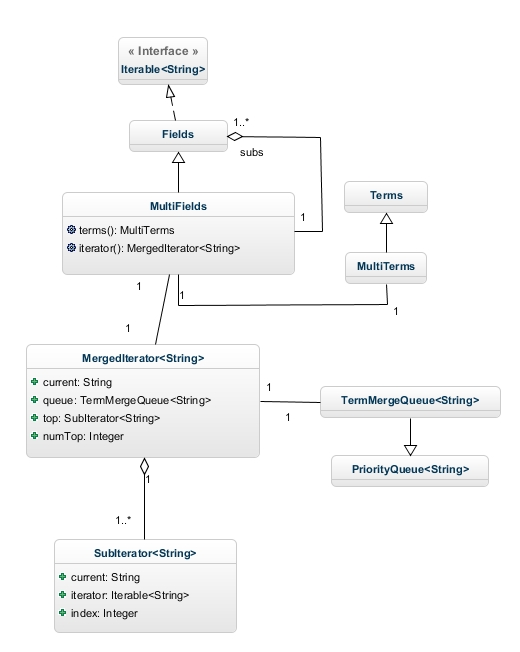
\includegraphics[scale=0.7]{MultiFields.jpg}
 \caption{\texttt{MultiFields} oraz klasy powiązane.}
\end{figure}

Z punktu widzenia algorytmu łączenia segmentów, najbardziej interesującymi metodami klasy \texttt{MultiFields} są \texttt{MultiFields.terms(String field)}, zwracająca termy należące do pola o podanej nazwie oraz \texttt{MultiFields.iterator()}, zwracająca iterator pozwalający na przechodzenie po kolejnych nazwach pól. 

\texttt{MultiFields.terms()} zwraca instancję typu \texttt{MultiTerms}, która podobnie jak \texttt{MultiTerms} agreguje wszystkie termy znajdujące się w danym polu. Ukrywa też to, że dla danego termu być może mamy do czynienia z kilkoma termami o takim samym tokenie, ale pochodzącymi z tego samego pola z różnych segmentów.

\texttt{MultiFields.iterator()} zwraca własną implementację iteratora napisów, \texttt{MergedIterator}. \texttt{MergedIterator} wykorzystuje kolejkę priorytetową do przechowywania zagregowanych iteratorów kolejności zdefiniowanej przez ich początkowe elementy. Dzięki temu 